\section{Unit Tests}

Unit tests are designed to ensure small pieces of
functionality within a larger system work as intended.
They are created by developers in tandem to the actual
code.
Some approaches, like test-driven development, require
tests to be written beforehand to ensure the code serves
the tests and vice-versa \parencite{softwareTesting}.

In \projectname{}, unit tests aim to test technical
functionality, such as logging or performance monitoring as
opposed to the business rules or constraints. Overall, 51
tests cover the backend code base as shown in 
Figure \ref{fig:unitTestRunner}.

\begin{figure}[h]
  \centering
  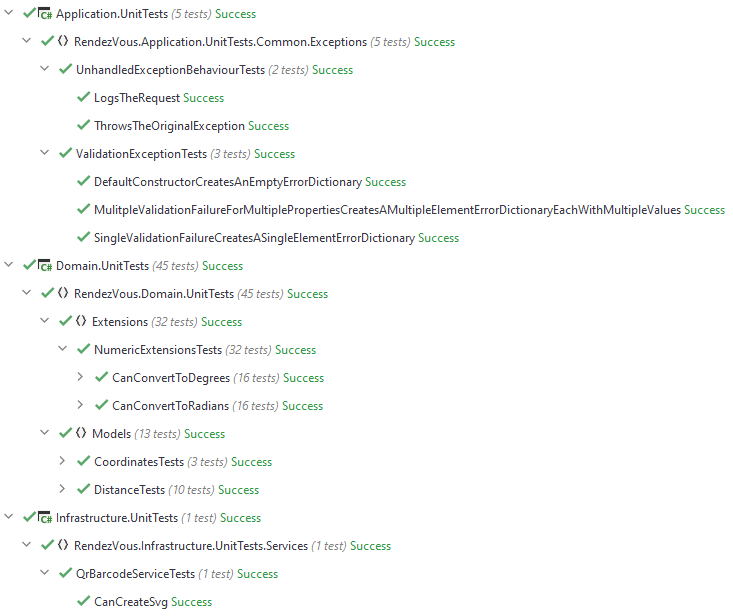
\includegraphics[width=0.9\linewidth]{07 testing/assets/unit/unit test runner.png}
  \caption{Unit Tests in the API}
  \label{fig:unitTestRunner}
\end{figure}

The NUnit testing framework provides the test runner, plus
a wide range of utilities to define additional behaviour.
For example, data-driven tests define a single test used on
a range of data provided with the
\lstinline{TestCaseSource} attribute.
Regular unit tests instead follow the \enquote{Arrange,
  Act, Assert} pattern for readability and consistency.
See Figure \ref{fig:unitTestStyles} for a comparison.

\begin{figure}[h]
  \centering
  \codesize

  \begin{subfigure}{\linewidth}
    \lstinputlisting{07 testing/assets/unit/aaa.cs}
    \caption{Behavioural}
  \end{subfigure}
  \begin{subfigure}{\linewidth}
    \lstinputlisting{07 testing/assets/unit/source.cs}
    \caption{Data-driven}
  \end{subfigure}

  \caption{Unit test styles}
  \label{fig:unitTestStyles}
\end{figure}
